\section{Introduction}
\label{sec:introduction}

AI systems increasingly produce candidate updates that may enter persistent operational records. Before admission, an output is a proposal whose origin, context, and uncertainty remain open to inspection. After admission, a value may drive reporting, payment, scheduling, or later automated decisions as a durable fact. The central systems question is therefore not merely whether a model produced a plausible value, but which authority made which value authoritative from which persisted proposal and record state.

Consider a record whose authoritative quantity is 90. A recognizer proposes \code{quantity=100}, but a reviewer authorizes 101; an unchanged batch-code field should retain its earlier source. The resulting record must preserve distinct statements: 90 was the predecessor value, the machine proposed $x_c=100$, and the human authorized the committed value $x_a=101$. Rewriting the candidate would falsely attribute 101 to the model; storing only the final value would erase the proposal that prompted the decision. Losing the unchanged field's source would leave the snapshot numerically intact but its lineage incomplete. A faithful admission history must therefore allow
\begin{equation}
x_c\neq x_a
\label{eq:intro-correction}
\end{equation}
while retaining both roles and the exact sources of the complete successor.

This problem arises in systems where people can correct AI-generated field candidates, accepted updates become persistent operational facts, and later review must reconstruct who authorized each value and where it came from. Authorized mutation changes an object that is already authoritative; correction-aware admission additionally preserves the relation between an untrusted proposal, a separate human decision, and the resulting authoritative record.

Existing systems address adjacent layers of this transition. Continuity Kernel separates off-commit candidates from atomic authoritative activation; LatticeMind treats conflict-aware claim selection and supersession as a write-time memory primitive; authority-collapse work studies loss of source authority during memory consolidation; MutMem binds cryptographically authorized changes to predecessor history; and MemTxn provides source-supported update and recovery boundaries \citep{he2026continuity,zhou2026latticemind,zhan2026authoritycollapse,saidi2026mutmem,cui2026memtxn}. Together, these mechanisms establish transaction, provenance, freshness, activation, and governed-memory foundations. This paper isolates correction-aware admission as the unit of analysis: an exact field candidate prompts a human decision that may authorize a different value, after which the system must construct a complete attributable record successor.

We introduce that relation as a correction-aware, field-level specialization of authoritative-state admission. Its semantic chain is
\begin{equation}
\begin{aligned}
\textit{exact candidate}
&\rightarrow\textit{candidate-bound human authorization}\\
&\rightarrow\textit{explicit authorized value}
\rightarrow\textit{complete successor}\\
&\rightarrow\textit{total field-source attribution}.
\end{aligned}
\label{eq:admission-chain}
\end{equation}
The candidate remains non-authoritative historical evidence; the authorization supplies authority for the value; and a trusted transaction constructs the successor. This representation-independent formulation specifies the observable distinctions a mechanism must preserve to separate the failure families considered here.

Five families define that characterization. Candidate identity and context distinguish equal-valued proposals that belong to different records, fields, evidence, or producers. Dual-value attribution distinguishes legitimate Correction from candidate erasure or false machine attribution. A freshness discriminator separates a current authorization from the same bytes replayed after supersession. A batch boundary distinguishes one atomic successor from fragmented commits that expose a partial intermediate state. Finally, a total per-field source relation distinguishes value-identical successors whose lineage is complete from successors whose sources are missing, replaced, duplicated, or ambiguous. We call this the \emph{failure-distinguishability} view of admission.

Our research question is:

\begin{quote}
Which authority-relevant distinctions let a system admit an AI-derived field candidate through an attributable human decision while preserving Correction, freshness, complete-record atomicity, and exact successor lineage?
\end{quote}

The central contribution is a contract that jointly relates an exact persisted proposal, a human-authorized value, and an atomic record successor with complete field-source attribution. Paired histories explain the design obligations: equal final values can conceal different authority roles, source relations, or commit groupings. We study this contract through \system{}, a Python/SQLite reference realization. C1--C2 specify the relation and its conditional information requirements; C3--C4 provide implementation and evaluation evidence:

\begin{enumerate}[label=\textbf{C\arabic*:},leftmargin=*]
  \item \textbf{Correction-aware admission contract.} We jointly specify exact candidate binding, human authority over an explicit value, and complete successor attribution. The relation preserves the proposal when $x_c\neq x_a$ and retains the prior sources of unchanged fields.
  \item \textbf{Conditional failure-distinguishability characterization.} Five paired histories identify information whose omission prevents separation of a corresponding safe/unsafe pair under the declared observation model. They provide explicit design checks for candidate substitution, false value attribution, stale replay, fragmented commits, and missing sources.
  \item \textbf{Relational and transactional realization.} We connect the contract to bounded Alloy assertions and encoding-sensitivity checks, a compare-and-swap-protected transaction, selected formal--concrete projections, and a production-facing fault catalogue.
  \item \textbf{Cost and agent-integration evaluation.} We measure persistence-equivalent admission costs and trace access, then evaluate a restricted proposal/verification surface across three qualified model configurations. Agent completion, acknowledgment, and recovery are assessed separately from host-enforced authority outcomes.
\end{enumerate}

The evaluation follows three questions in this dependency chain: which information is needed to distinguish admission failures (RQ1--RQ2), whether the transaction preserves these relations in persisted executions (RQ3--RQ5), and what costs and agent-integration behavior arise in the reference realization (RQ6--RQ8). Two bounded Alloy profiles, concrete projections and fault tests, fixed-grid measurements, and a repeated live-agent benchmark supply the corresponding evidence. \Cref{fig:admission-workflow} gives an overview of the proposal, review, and admission boundary.

% FIGURE SOURCE: exact author-approved Canva design DAHUNAr-imw export. The PDF is the manuscript source; a matching converted SVG is retained beside it for downstream reuse.
\begin{figure*}[t]
\centering
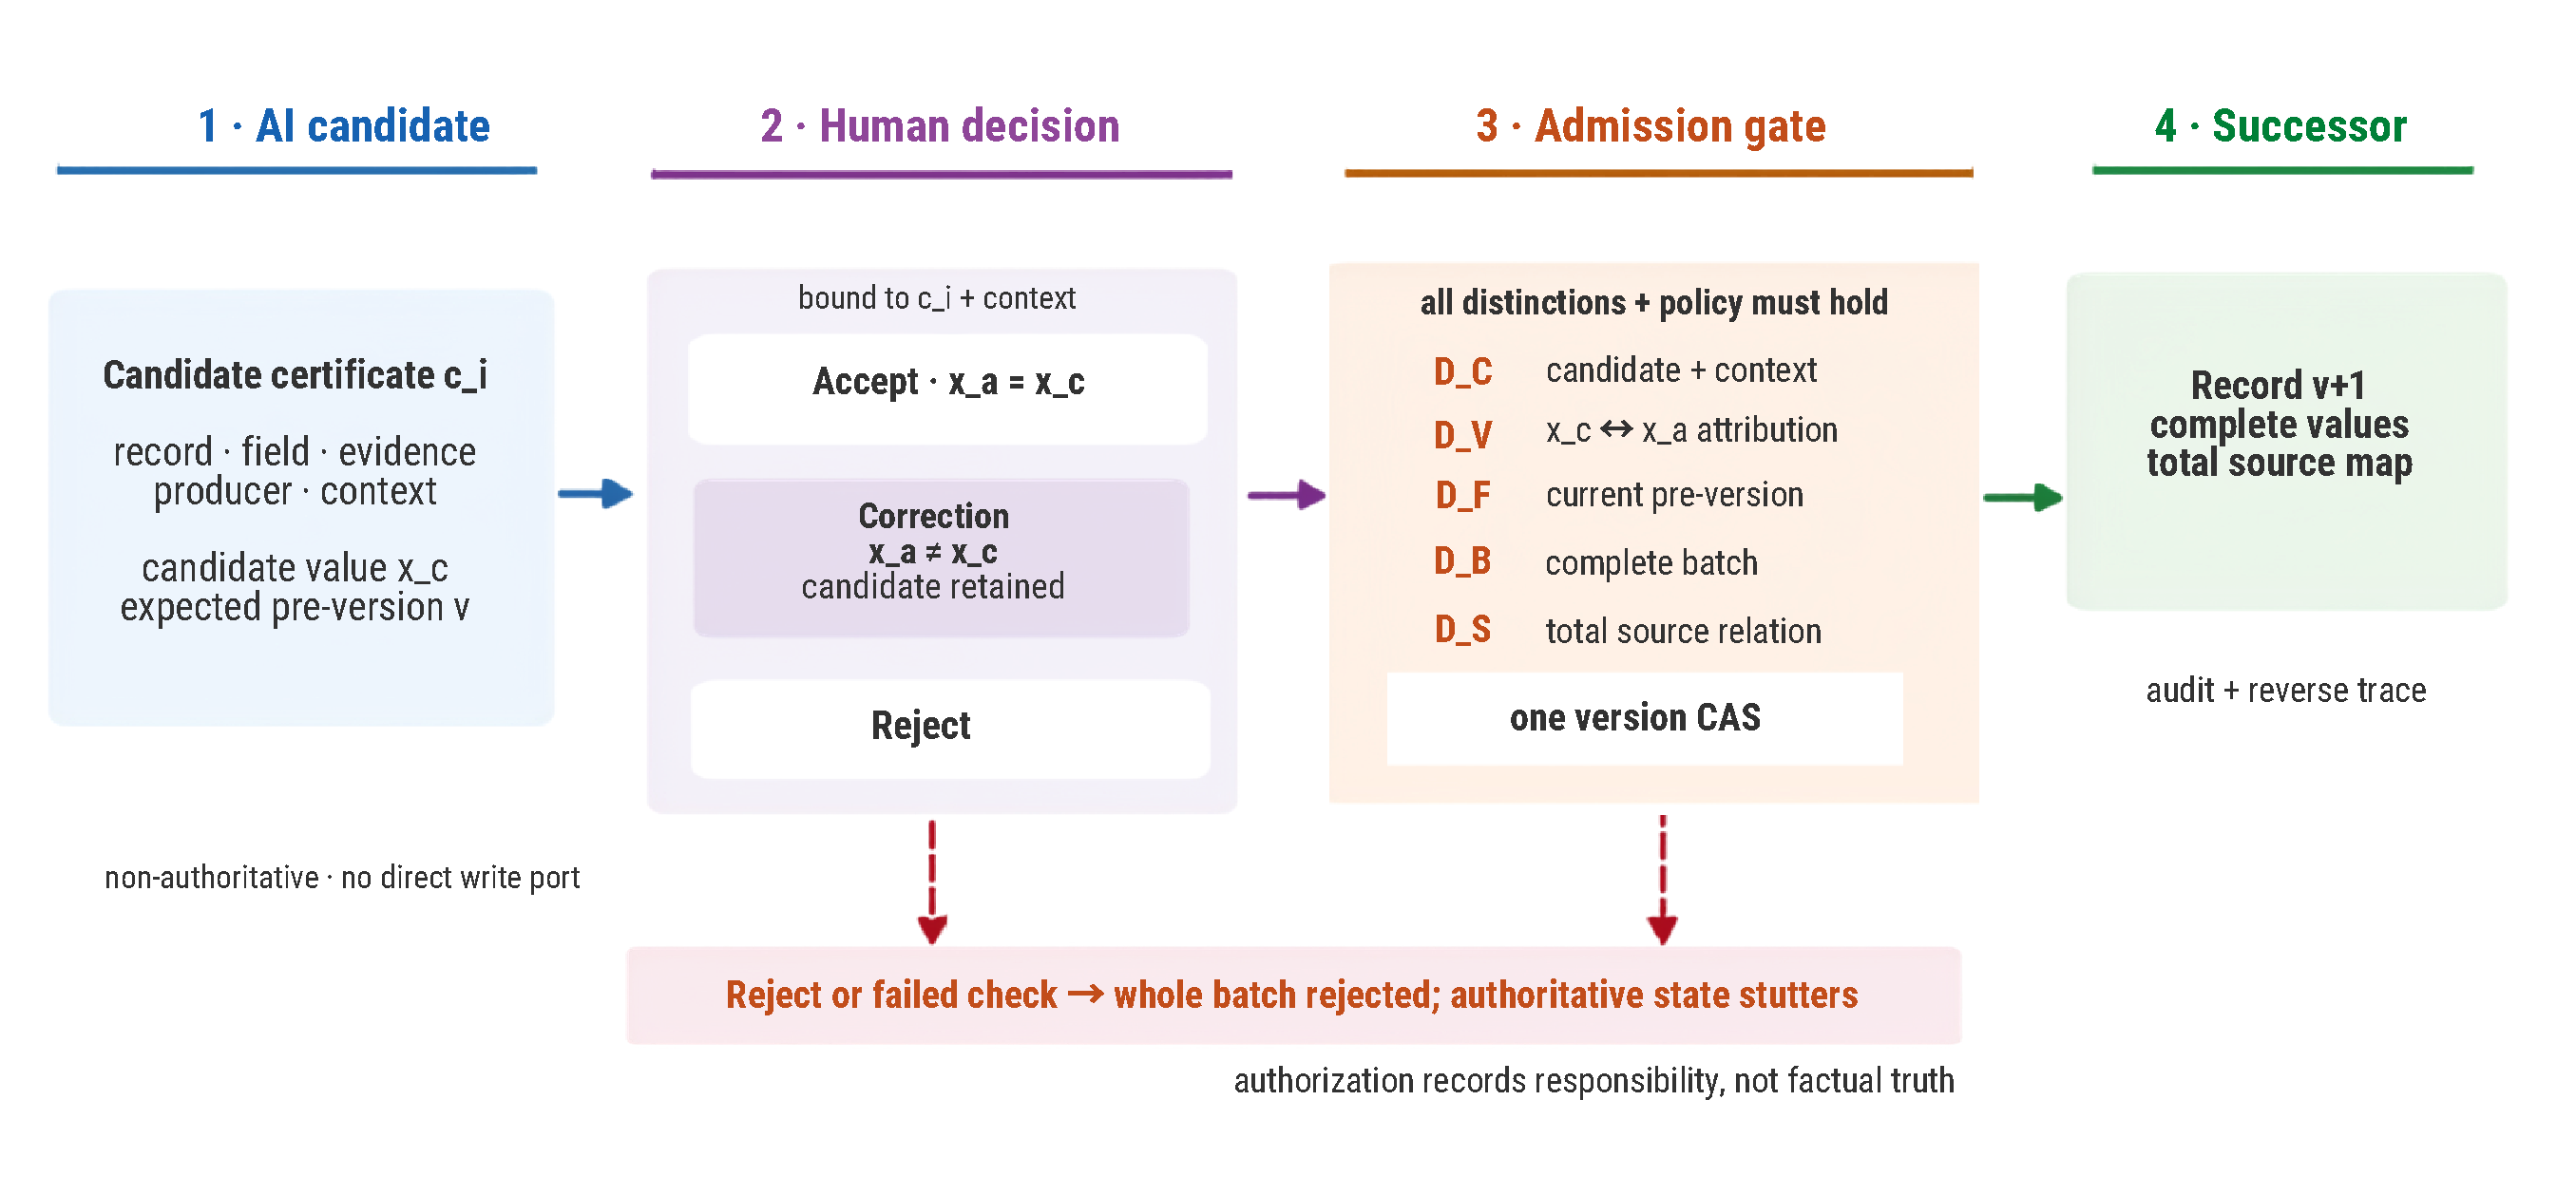
\includegraphics[width=0.96\textwidth]{figures/canva/admission-workflow-canva.pdf}
\caption{Correction-aware authoritative-state admission. A persisted AI candidate has no direct authoritative write port. A candidate-bound human decision may Accept the proposed value, Correct it while retaining the exact candidate, or Reject it. Admission succeeds only when the five distinction classes and principal policy hold; one version compare-and-swap then creates a complete successor and total source map. Reject or failed validation leaves the authoritative state unchanged.}
\label{fig:admission-workflow}
\end{figure*}

The remainder of the paper positions the abstraction against its nearest neighbors (\cref{sec:related}), defines the observation model and admission contract (\cref{sec:contract}), presents the bounded and concrete realizations (\cref{sec:alloy,sec:realization}), explains their selected correspondence (\cref{sec:conformance}), and reports the evaluation (\cref{sec:evaluation,sec:results}) before discussing inference boundaries (\cref{sec:discussion}).
